% ------------------------------------------------------------------
%  Section: the interaction-driven pi junction at g = 0 (Fig. junctions)
%  Data: data/ephi_Nr10_tJ0.5_A.json, data/bench/ephi_Nr10_U2_tJ0.5.json, data/ephi_even_fine_*.json;
%  figure: code/make_figures.py (fig_junctions)
% ------------------------------------------------------------------
\paragraph*{Interaction-driven $\pi$ junction.}
We first characterize the junction alone ($g=0$). DMRG in the even and odd fermion-parity
sectors [Fig.~\ref{fig:junctions}(b,c)] gives the $0$--$\pi$ transition known for magnetic quantum
dots~\cite{GlazmanMatveev1989,SpivakKivelson1991,Vecino2003,Karrasch2008,vanDam2006,Cleuziou2006,Delagrange2015}.
For small $U$ the singlet (even) state is the ground state at every phase and the junction is a
$0$-junction; for large $U$ the Kramers doublet (odd sector) is the ground state at every phase and
$E(\varphi)$ has its \emph{minimum} at the Cooper-pair phase $\pi$ (electron phase $\varphi=\pi/2$).
At $U=2\Delta$ we find $E_2=+7.39\times10^{-3}\Delta$ with $|E_1|/E_2=2\%$ and
$|E_4|/E_2<1\%$: a pure $\pi$ junction, indistinguishable after normalization from the
half-flux-biased weak link [Fig.~\ref{fig:junctions}(a)]. The $\pi$ coupling decreases
monotonically with $U$ ($E_2\propto U^{-1.3}$ for $4\Delta\le U\le8\Delta$), as expected for
cotunnelling through the singly occupied level.

Three crossings of the two sectors matter below, and they are distinct
[Fig.~\ref{fig:junctions}(b)]. The zero-flux crossing $U_c^0=0.94\Delta$ is the $0$--$\pi$
transition of the junction itself, where $E_{\rm odd}(0)=E_{\rm even}(0)$. The crossing of the
\emph{global} minima of the two surfaces, $E_{\rm odd}(\pi/2)=E_{\rm even}(0)$, lies lower, at
$0.85\Delta$, because the doublet surface has its minimum at half a flux quantum while the singlet
surface has it at zero. In between, $0.85\Delta<U<U_c^0$, the junction is a $0$-junction at zero flux
although the lowest state of the ring at \emph{any} flux is the doublet: a loop in which the flux
is free to adjust can switch to the doublet by letting a flux $\Phi_0/2$ in. This is what the mode
does above a finite coupling, and it moves the boundary $U_c(g)$ of the loop into this window
(next section). Finally, the singlet surface itself has a cusp at $\varphi=\pm\pi/2$
[dotted line in Fig.~\ref{fig:junctions}(a)]: at half a flux quantum two even-parity states cross
so that $E_{\rm even}(\varphi)$ cannot
be represented by a few harmonics of Eq.~\eqref{eq:harm}. The doublet surface, in contrast, is a
smooth $\cos2\varphi$ with $2\%$ corrections.

% ------------------------------------------------------------------ figure
\begin{figure*}
  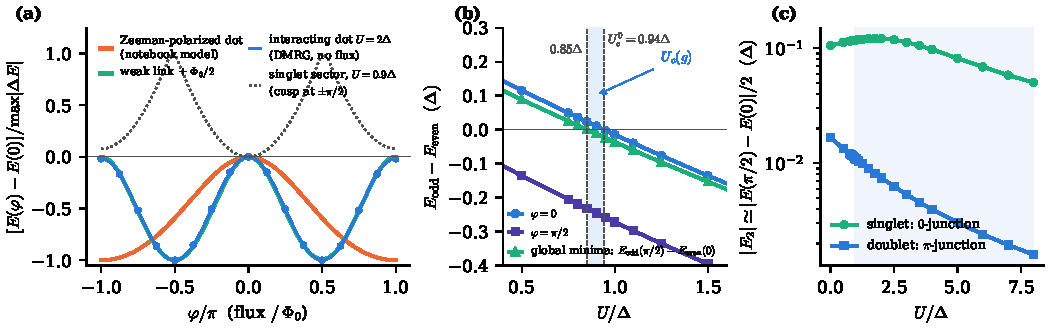
\includegraphics[width=\textwidth]{../figs/fig_junctions.pdf}
  \caption{\label{fig:junctions}%
  (a) Normalized ground-state energy of the loop versus the electron phase
  $\varphi$ (flux in units of $h/2e$) for three junctions:
  Zeeman-polarized dot in a short ring (dominated by the single-electron
  harmonic $\cos\varphi$), an ordinary weak link biased by $\Phi_0/2$ ($L=14$), and an
  interacting dot at $U=2\Delta$ without any bias ($L=10$; DMRG, symbols; line: cosine fit).
  Dotted: the singlet (even-sector) surface at $U=0.9\Delta$, with its cusp at $\pm\pi/2$.
  (b) Parity competition $E_{\rm odd}-E_{\rm even}$ of the interacting-dot
  ring at $\varphi=0$, at $\varphi=\pi/2$, and between the global minima of the two surfaces
  (DMRG, $L=10$, $\Delta=t$, $t_J=0.5\Delta$). The zero-flux crossing $U_c^0=0.94\Delta$ and the crossing
  of the global minima at $0.85\Delta$ bound the window (shaded) in which the boundary $U_c(g)$ of the
  loop moves with the coupling to the mode.
  (c) Josephson energy $|E_2|$ in the singlet ($0$) and doublet ($\pi$)
  sectors. Shading: doublet ground state at zero flux.}
\end{figure*}
